\chapter{Adversarial Attacks to Data-Driven Control}\doublespacing % Main chapter title
\label{chap:attacks} % Change X to a consecutive number; for referencing this chapter elsewhere, use \ref{ChapterX}
This chapter evaluates the robustness of direct data-driven control methods against adversarial attacks. %, and to provide insights on how to design secure and reliable data-driven controller design algorithms.
The objective of the attacker is to disrupt the stability of the system by making small perturbations to the data.
% These small perturbations to the data and disrupts the stability of the closed-loop system.
It is assumed that the attacked has complete knowledge of the system.
% As the worst-case scenario, we first consider a powerful attacker who has complete knowledge of the system, the controller design algorithm, and the clean input and output data. Subsequently, we consider gray box attacks where we assume that the adversary has access to the model and the algorithm but not the data, and additionally may not know design parameters in the algorithm.
\begin{definition}[Transferability Property]
Transferability property is the effectiveness of adversarial perturbations without partial knowledge.
\end{definition}
\begin{definition}[Transferability across data]
Effectiveness of the attack without the knowledge of data.
\end{definition}
\begin{definition}[Transferability across parameters]
Effectiveness of the attack without the knowledge of parameters.
\end{definition}
Before delving into security, let us discuss the standard algorithms for optimal feedback.
\section{Linear Quadratic Regulator}% based on Fundamental Lemma}
\label{subsec:data-driven}
% We first review the direct data-driven control based on the Willems' fundamental lemma~\cite{Persis2020}.
% using the notation from~\cite{Dorfler2022On}.
% Consider a discrete-time linear time-invariant system
% $x(t+1)=Ax(t)+Bu(t)+d(t)$ for $t\in\mathbb{N}$
% %\[
% % x(t+1)=Ax(t)+Bu(t)+d(t),\quad t\in\mathbb{N}
% %\]
% where $x(t)\in\mathbb{R}^n$ is the state, $u(t)\in\mathbb{R}^m$ is the control input, and $d(t)\in\mathbb{R}^n$ is the exogenous disturbance.
We consider the standard model as discussed in \ref{sec:stability informativity}.

Consider the linear quadratic regulator (LQR) problem, where the pair $(A,B)$ is unknown to the designer but it is known to be stabilizable.
% We consider the linear quadratic regulator (LQR) problem, which has widely been studied as a benchmark problem.
Now, the objective is to design as state-feedback control that minimizes the cost function
\begin{equation}
J(K)=\sum_{i=1}^n\sum_{t=0}^{\infty} \{x(t)^\top Qx(t) + u(t)^\top Ru(t)\}|_{x(0)=e_i}
\end{equation}
%\[
% \textstyle{J(K)=\sum_{i=1}^n\sum_{t=0}^{\infty} \{x(t)^{\sf T}Qx(t) + u(t)^{\sf T}Ru(t)\}}|_{x(0)=e_i}
%\]
where $Q\geq 0$, $R> 0$ and $e_i$ is the $i$th standard  basis vector.

This cost function can be rewritten as
\begin{equation}
J(K)=\trace(QP)+\trace(K^\top RKP)
\end{equation}
%\[
% J(K)=\trace(QP)+\trace(K^{\sf T}RKP)
%\]
where $P\geq I$.

We will follow the previous notation for data matrices containing signals values of $\bmu, \bmx$.
%\[
% \begin{array}{ll}
%  U_- \hs :=[u(0)\ u(1)\ \cdots u(T-1)]\in \mathbb{R}^{m\times T}\\
%  X \hs :=[x(0)\ x(1)\ \cdots x(T-1)\ x(T)] \in \mathbb{R}^{n\times (T+1)}
% \end{array}
%\]
% are available.
% The first and last $T$-long time series of $X$ are denoted by $X_-\in \mathbb{R}^{m\times T}$ and $X_+\in \mathbb{R}^{m\times T},$ respectively.
Let the disturbance signal be $\bmd$ and its data matrix be $D_0:=[d(0)\ d(1)\ \cdots\ d(T-1)]\in \mathbb{R}^{m\times T}$.
%\[
% D_0:=[d(0)\ d(1)\ \cdots\ d(T-1)]\in \mathbb{R}^{m\times T},
%\]
% Now,
% %$X_+-D_0=[B\ A]W_0$
% \[
%  X_+-D_0 = \bbm B& A\ebm W_0\qquad \text{where $W_0:=\bbm U_-\\X_-\ebm$}
% \]

%\[
% X_+-D_0 = [B\ A]
% W_0,\quad W_0:=
% \left[\hspace{-1mm}
% \begin{array}{c}
% U_-\\
% X_-
% \end{array}\hspace{-1mm}
% \right].
%\]
% We here assume that ${\rm rank}\, W_0 = n+m$
%\[
% {\rm rank}\, W_0 = n+m
%\]
% holds.
% This rank condition, which is generally necessary for data-driven LQR design, is satisfied if the input signal is persistently exciting in the noiseless case as shown by the Willems' fundamental lemma~\cite{willems2005note}.
We will assume that Willem's fundamental lemma is satisfied which enables us to carry out data-driven control.

\begin{lemma}{\rm \cite{Persis2020,Dorfler2022On}, LQR controller design}
The noise free algorithm is given by
\begin{equation}\label{eq:prob_ori}
\begin{array}{cl}
 \displaystyle{\min_{P,K,G}} & \trace(QP)+\trace(K^\top RKP)\\
 {\text{such that}} & X_+GPG^\top X_+^\top -P+I\preceq 0,\  P \succeq I\ {\text{ and }} \bbm K\\ I^\top\ebm=\bbm U_-\\X_-\ebm G\\
%  & \left[\hspace{-1mm}
% \begin{array}{c}
% K\\
% I
% \end{array}\hspace{-1mm}
% \right]=W_0G.
\end{array}
\end{equation}
\end{lemma}
% The key idea of the approach laid out in~\cite{Persis2020} is to parameterize the controller using the available data by introducing a new variable $G\in\mathbb{R}^{T\times n}$ with the relationship
% \begin{equation}\label{eq:KI}
% % \left[\hspace{-1mm}
% % \begin{array}{c}
% % K\\
% % I
% % \end{array}\hspace{-1mm}
% % \right]
% [K^{\sf T}\ I]^{\sf T}
% =W_0G.
% \end{equation}
% %with a matrix $G\in\mathbb{R}^{T\times n}$.
% Then the closed-loop matrix can be parameterized directly by data matrices as
% $A+BK = [B\ A]W_0G = (X_+-D_0)G.$
% %\[
% %\begin{array}{ll}
% % A+BK \hs = [B\ A]W_0G\\
% %  \hs = (X_+-D_0)G.
% %\end{array}
% %\]
% The LQR controller design can be formulated as
% %Using this new parameterization, the LQR problem can be expressed as
% %\[
% %\begin{array}{cl}
% % \displaystyle{\min_{P,K,G}} & \trace(QP)+\trace(K^{\sf T}RKP)\\
% % {\rm s.t.} & (X_+-D_0)GPG^{\sf T}(X_+-D_0)^{\sf T}-P+I\preceq 0\\
% %  & P \succeq I\\
% %  & \left[\hspace{-1mm}
% % \begin{array}{c}
% % K\\
% % I
% % \end{array}\hspace{-1mm}
% % \right]=W_0G
% %\end{array}
% %\]
% %with optimal control gain $K=U_0G$.
% %Since $D_0$ is unknown, a natural approach is to disregard $D_0$ with the formulation
% \begin{equation}\label{eq:prob_ori}
% \begin{array}{cl}
%  \displaystyle{\min_{P,K,G}} & \trace(QP)+\trace(K^{\sf T}RKP)\\
%  {\rm s.t.} & X_+GPG^{\sf T}X_+^{\sf T}-P+I\preceq 0\\
%   & P \succeq I\ {\rm and}\ \eqref{eq:KI}\\
%   & 
% %  & \left[\hspace{-1mm}
% % \begin{array}{c}
% % K\\
% % I
% % \end{array}\hspace{-1mm}
% % \right]=W_0G.
% \end{array}
% \end{equation}
% by disregarding the noise term.
% %which can be reformulated into a convex program~\cite{Dorfler2021Certainty}.
For a robust approach, a regularized optimiser is proposed.
% However, it has been revealed that the formulation~\eqref{eq:prob_ori} is not robust to disturbance~\cite{Dorfler2022On}.
% To enhance robustness against disturbance, a regularized formulation has been proposed:
\begin{equation}\label{eq:prob_reg1}
\begin{array}{cl}
 \displaystyle{\min_{P,K,G}} & \trace(QP)+\trace(K^\top RKP)+\gamma\|\Pi G\|\\
 \text{ such that} & X_+GPG^\top X_+^\top -P+I\preceq 0,\ P \succeq I\ \text{ and } \bbm K\\ I^\top\ebm=\bbm U_-\\X_-\ebm G\\
%  & \left[\hspace{-1mm}
% \begin{array}{c}
% K\\
% I
% \end{array}\hspace{-1mm}
% \right]=W_0G
\end{array}
\end{equation}
where $\gamma\geq0$, $\Pi:=I-W_0^{\dagger}W_0$
%\[
% \Pi:=I-W_0^{\dagger}W_0
%\]
and $\|\cdot\|$ is any matrix norm.
% The regularizer $\gamma\|\Pi G\|$ is referred to as certainty-equivalence regularization because it leads to the controller equivalent to the certainty-equivalence indirect data-driven LQR with least-square estimation of the system model when $\gamma$ is sufficiently large~\cite{Dorfler2022On}.
% Meanwhile, another regularization that can guarantee robustness has been proposed:
% \begin{equation}\label{eq:prob_reg2}
% \begin{array}{cl}
%  \displaystyle{\min_{P,K,G}} & \trace(QP)+\trace(K^{\sf T}RKP)+\rho\,\trace(GPG^{\sf T})\\
%  {\rm s.t.} & X_+GPG^{\sf T}X_+^{\sf T}-P+I\preceq 0\\
%   & P \succeq I\ {\rm and}\ \eqref{eq:KI}\\
% %  & \left[\hspace{-1mm}
% % \begin{array}{c}
% % K\\
% % I
% % \end{array}\hspace{-1mm}
% % \right]=W_0G
% \end{array}
% \end{equation}
% with a constant $\rho\geq0$.
% The regularizer $\rho\,\trace(GPG^{\sf T})$ plays the role to reduce the size of the matrix $GPG^{\sf T}$ to achieve the actual stability requirement $(X_+-D_0)GPG^{\sf T}(X_+-D_0)^{\sf T}-P+I\preceq 0$ using the constraint $X_+GPG^{\sf T}X_+^{\sf T}-P+I\preceq 0$.
% We refer to the latter one as robustness-inducing regularization.
% For reformulation of~\eqref{eq:prob_ori},~\eqref{eq:prob_reg1}, and~\eqref{eq:prob_reg2} into convex programs, see~\cite{Dorfler2021Certainty}.
\section{Threat Model}
The description of threat model is as follows (and shown in \ref{fig:scenario})
\begin{itemize}
\item A perturbation $(\Delta U, \Delta X)$ can be added to the input and output data
\item The system model $(A,B)$ and the design algorithms are known to the attacker
\end{itemize}
The controller designed using perturbed data $\hat{K}$ leads to a different system matrix $A+B\hat{K}$. Now, if the eigenvalues of $A+B\hat{K}$ perturb outside the unit circle then the system is destabilised.
% The controller $\hat{K}$ is designed using the perturbed data $(\hat{U},\hat{X}):=(U_0+\Delta U,X+\Delta X)$, which results in the closed-loop matrix $A+B\hat{K}$.
% The attack objective is to destabilize the system by crafting a small perturbation such that the closed-loop matrix has an eigenvalue outside the unit circle.
\begin{figure}[H]
  \centering
  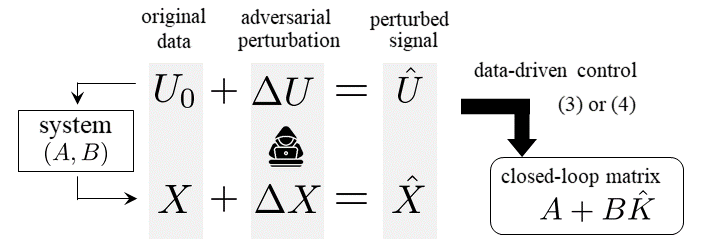
\includegraphics[width=0.6\linewidth]{scenario.png}
  \caption{\cite{10383531}, Threat model
  % The adversary is able to add a perturbation $(\Delta U, \Delta X)$ to the original input and output data $(U_0,X)$ with knowledge of the system model, the signals, and the controller design algorithm.
  % The controller $\hat{K}$ is designed using the perturbed data $(\hat{U},\hat{X})$, which results in the closed-loop matrix $A+B\hat{K}$.
  }
  \label{fig:scenario}
\end{figure}
% Additionally, we consider gray-box attacks where the adversary has access to the system model $(A,B)$ and the controller design algorithm but not the data $(U_0,D_0,X)$, and additionally may not know the design parameters $\gamma$ and $\rho$.
% In this case, a reasonable attack strategy is to use hypothetical input $\hat{U}$ and disturbance $\hat{D}_0$ and calculate the corresponding state trajectory $\hat{X}$.
% We refer to effectiveness of the attack without knowledge of the data as \emph{the transferability across data.}
% Additionally, when the design parameters are unknown, hypothetical design parameters $\hat{\gamma}$ or $\hat{\rho}$ are also used.
% We refer to the effectiveness in this scenario as \emph{the transferability across parameters.}
% We numerically evaluate the transferability properties in Sec.~\ref{sec:ex}.	
\section{Fast Gradient Sign Method}
\cite{Goodfellow2015Explaining} developed the fast gradient sign method (FGSM) to compute adversarial perturbations for given images efficiently. For a loss function of the neural network given by $L(X,Y;\theta)$, $X\in\mathcal{X}$ is the input, $Y\in\mathcal{Y}$ is the label, and $\theta$ is the trained parameter. And $f:\mathcal{X}\to\mathcal{Y}$ is the trained classification model. 

The aim of the attacker is to add small perturbations to cause misclassification in the model.
% Specifically, the max norm of the perturbation is restricted, i.e., $\|\Delta\|_{\rm max} \leq \epsilon$
% $\Delta\in\{\Delta\in\mathcal{X}: \|\Delta\|_{\rm max} \leq \epsilon \}$
% with a small constant $\epsilon>0$.
This perturbation are designed in such a way that they locally maximises the loss function. This can be done by choosing a perturbation parallel to the direction of gradient of the loss function which is approximated using a linear approximation
% The linear approximation of the loss function with respect to $\Delta$ is given by
\begin{equation}\label{eq:FGSM_linear_approx}
 L(X+\Delta,Y;\theta)\approx L(X,Y;\theta)+\sum_{i,j}(\nabla_{X}L(X,Y;\theta))_{i,j}\Delta_{i,j}\rightarrow \Delta = \epsilon\, {\rm sign}(\nabla_{X}L(X,Y;\theta))
\end{equation}
where the subscript $(\cdot)_{i,j}$ denotes the $(i,j)^{th}$ component.
% The right-hand side of~\eqref{eq:FGSM_linear_approx} is maximized by choosing $\Delta_{i,j}=\epsilon\,{\rm sign}(\nabla_{X}L(X,Y;\theta))_{i,j}$, whose matrix form is given by
% \[
%  \Delta = \epsilon\, {\rm sign}(\nabla_{X}L(X,Y;\theta)).
% \]
%Its core idea is to choose each element of the perturbation such that the loss function increases.
% FGSM creates a series of perturbations in the form increasing $\epsilon$ until misclassification occurs.
% In the next section, we apply this idea to adversarial attacks on direct data-driven control for destabilization.
\section{Directed Gradient Sign Method}
\cite{10383531} developed the directed gradient sign method (DGSM) using similar principles as FGSM. It designs a perturbation such that the eigenvalues are shifted in less stable direction. It is calculated using linear approximations of eigenvalues as follows
%\[
% \Delta:=(\Delta U, \Delta X).
%\]
%Let
%$\Lambda:\mathbb{R}^{m\times T}\times \mathbb{R}^{n\times(T+1)} \times \mathbb{R}^{(m+n)\times (2T+1)}\to\mathbb{C}^n$
%\[
% \Lambda:\mathbb{R}^{m\times T}\times \mathbb{R}^{n\times(T+1)} \times \mathbb{R}^{(m+n)\times (2T+1)}\to\mathbb{C}^n
%\]
%be the map from the obtained data $(U_0,X)$ with the perturbation $(\Delta U, \Delta X)$ to the eigenvalues of the resulting closed-loop system $(\lambda_1,\ldots,\lambda_n)$ with the direct data-driven control~\eqref{eq:prob_reg1} or~\eqref{eq:prob_reg2}.
%Specifically,
% Let
% %$\Lambda(U_0,X,\Delta):=\sigma(A+B\hat{K})$
% \[
%  \Lambda(U_0,X,\Delta):=\sigma(A+B\hat{K})
% \]
% denote the eigenvalues of the closed-loop system with the direct data-driven control~\eqref{eq:prob_reg1} or~\eqref{eq:prob_reg2} using the perturbed data $(\hat{U},\hat{X})$.
% %where $\hat{K}$ is designed using the perturbed data $(\hat{U},\hat{X})$.
% The aim of the attack is to place some element of $\Lambda(U_0,X,\Delta)$ outside the unit circle.
\begin{equation}\label{eq:DGSM_linear_approx}
 \lambda_i(U_0,X,\Delta)\simeq \lambda_i(U_0,X,0)+\sum_{i,j} \nabla_{\Delta}\lambda_i(U_0,X,\Delta)) \Delta_{i,j}.
\end{equation}
$\Delta_{i,j}$ is chosen such that the right-hand side of~\eqref{eq:DGSM_linear_approx} moves closer to the unit circle.
Hence, 
\[
 \Delta = \epsilon\, {\rm sign}(\Pi_{\lambda_i}(\nabla_{\Delta}\lambda_i(U_0,X,\Delta)))
\]
where 
\begin{equation}\label{eq:Pi}
 \Pi_{\lambda_i}(Z):= \Real{\lambda_i}\Real{Z}+\Imag{\lambda_i}\Imag{Z} \quad \text{and} \quad Z:=\nabla_{\Delta}\lambda_i(U_0,X,\Delta)
\end{equation}

Figure \ref{fig:vuln_ins} demonstrates the working of DGSM
\begin{figure}[H]
  \centering
  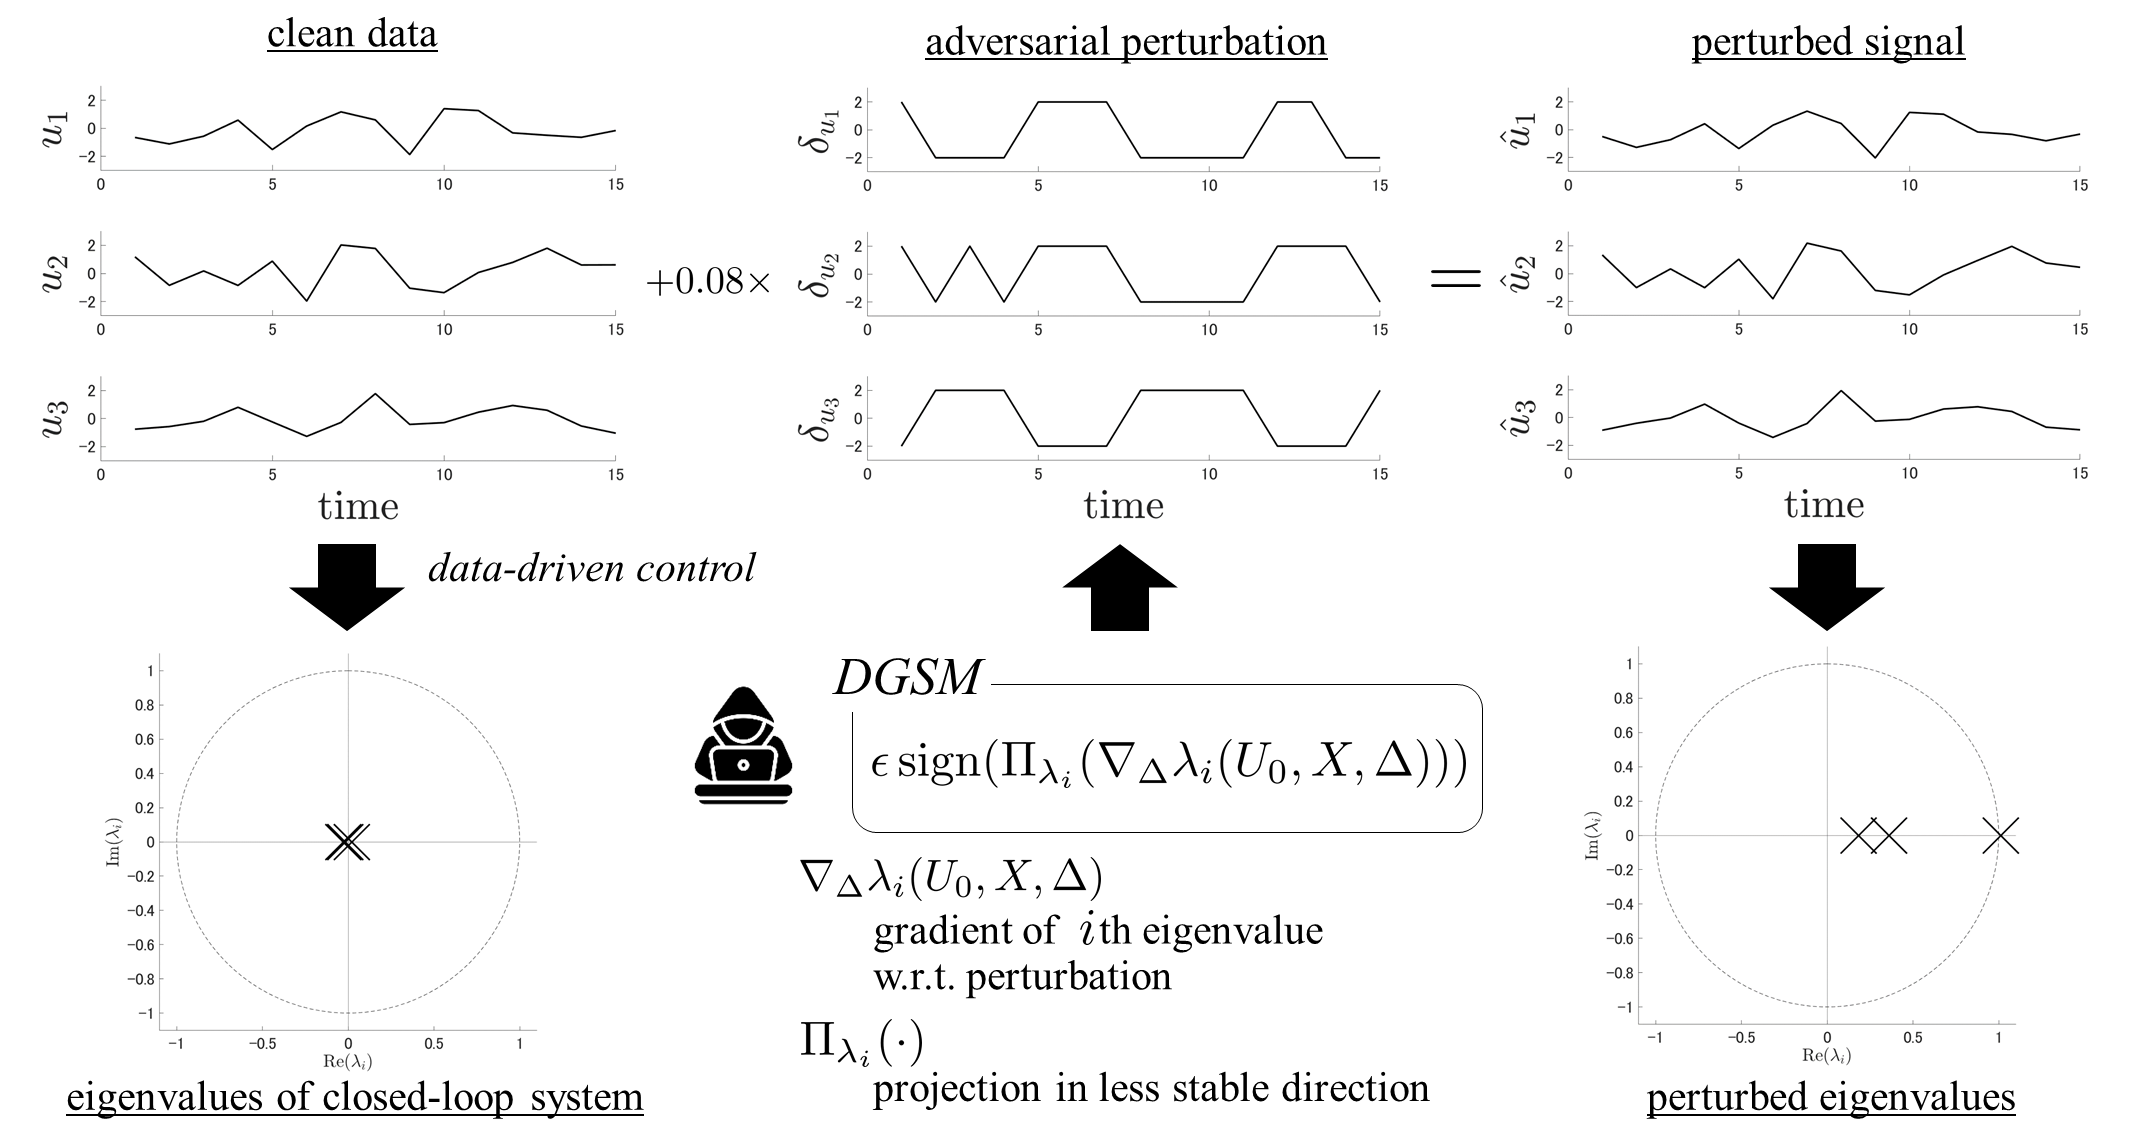
\includegraphics[width=0.98\linewidth]{vulnerable_instance.png}
  \caption{\cite{10383531}, 
  Overview of DGSM, using a discrete-time linear system% with three-dimensional input
  % The adversarial perturbation created by DGSM is added to the original signal, but the perturbed signal appears almost identical to the original one.
  % Nevertheless, the resulting closed-loop system obtained through direct data-driven control with a regularizer becomes unstable due to the adversarial attack.
  % Indeed, the eigenvalues of the closed-loop system with the clean data are $\{-0.0177, 0.0212, -0.0275\}$, while those with the perturbed data are $\{0.1824, 0.3613, 1.0120\}$.
  % The specific parameters of this instance are provided in Appendix.
  % Note that the output signal is also perturbed but its illustration is omitted for clarity.
  }
  \label{fig:vuln_ins}
\end{figure}
% The core idea of DGSM is to choose a perturbation that locally shifts an eigenvalue in the less stable direction.
% %the gradient of an eigenvalue moves in the less stable direction.
% We temporarily fix the eigenvalue of interest, denoted by $\lambda_i(U_0,X,\Delta)$,
% and denote its gradient with respect to $\Delta$ by $\nabla_{\Delta}\lambda_i(U_0,X,\Delta)$.

% %We hereinafter focus on a single eigenvalue $\lambda_i$, and let $\lambda_i(U_0,X,\Delta)$ be the $i$th element of $\Lambda(U,X,\Delta)$.
% %We denote the gradient of $\lambda_i(U_0,X,\Delta)$ with respect to $\Delta$ by $\nabla_{\Delta}\lambda_i(U_0,X,\Delta)$.
% %The aim of the attack is to place $\lambda_i(U_0,X,\Delta)$ outside the unit circle.
% %The core idea of DGSM is to choose a perturbation such that the gradient moves in the less stable direction.
% The linear approximation of the eigenvalue with respect to $\Delta$ is given by
% \begin{equation}\label{eq:DGSM_linear_approx}
%  \lambda_i(U_0,X,\Delta)\simeq \lambda_i(U_0,X,0)+\sum_{i,j} \nabla_{\Delta}\lambda_i(U_0,X,\Delta)) \Delta_{i,j}.
% \end{equation}
% We choose $\Delta_{k \ell}$ such that the right-hand side of~\eqref{eq:DGSM_linear_approx} moves closer to the unit circle.
% Specifically, DGSM crafts the perturbation
% \[
%  \Delta = \epsilon\, {\rm sign}(\Pi_{\lambda_i}(\nabla_{\Delta}\lambda_i(U_0,X,\Delta)))
% \]
% where $\Pi_{\lambda_i}:\mathbb{C}^{(m+n)\times(2T+1)}\to \mathbb{R}^{(m+n)\times(2T+1)}$ is defined by
% \begin{equation}\label{eq:Pi}
%  \Pi_{\lambda_i}(Z):= \Real{\lambda_i}\Real{Z}+\Imag{\lambda_i}\Imag{Z}
% \end{equation}
% with
% %$Z:=\nabla_{\Delta}\lambda_i(U_0,X,\Delta).$
% \[
%  Z:=\nabla_{\Delta}\lambda_i(U_0,X,\Delta).
% \]
% %for $Z\in\mathbb{C}^{(m+n)\times(2T+1)}$.
\begin{figure}[H]
  \centering
  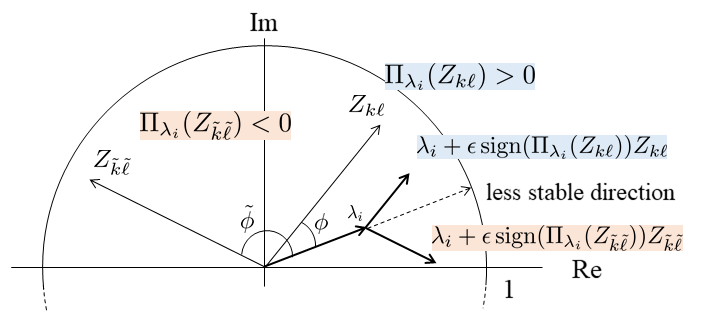
\includegraphics[width=0.4\linewidth]{Pi.png}
  \caption{\cite{10383531}, Role of the function $\Pi_{\lambda_i}$ in~\eqref{eq:Pi}
  % for scalar variables $z$ and $\tilde{z}$.
  % Since $Z_{i,j}$ faces the direction of $\lambda_i$, the angle $\phi$ between $\lambda_i$ and $Z_{i,j}$ is less than $\pi/2$, which leads to $\Pi_{\lambda_i}(Z_{i,j})>0$.
  % On the other hand, since $\tilde{\phi}$ between $\lambda_i$ and $Z_{\tilde{k}\tilde{\ell}}$ is greater than $\pi/2$, $\pi_{\lambda_i}(Z_{\tilde{k}\tilde{\ell}})<0$.
  % As a result, in both cases, the perturbed eigenvalue moves closer to the unit circle.
  }
  \label{fig:Pi}
\end{figure}
As shown in \ref{fig:Pi}, the perturbed eigenvalue moves closer to the exterior irrespective of its direction.
The perturbed eigenvalue $\hat{\lambda}_i$ can be approximated by 
%If $\epsilon$ is sufficiently small, the perturbed eigenvalue $\hat{\lambda}_i$ can be approximated by
\[
 \textstyle{\hat{\lambda}_i\simeq\lambda_i+\epsilon\,\sum_{i,j}\text{ sign}(\Pi_{\lambda_i}(Z_{i,j}))Z_{i,j},}
\]
and as $\epsilon$ increases, this eigenvalue moves outside of the circle

DGSM uses this idea in an iterative fashion to calculate the smallest $\epsilon$ which destabilises the system from a given set.
% DGSM performs the procedure above for every $\lambda_i$ for $i=1,\ldots,n$ increasing $\epsilon$ until the resulting system is destabilized.
% Its algorithm is summarized in Algorithm~1, where $\{\epsilon_k\}$ denotes possible candidates of the constant $\epsilon$ in the ascending order.
% Algorithm~1 finds a perturbation $\Delta$ with the smallest $\epsilon$ in $\{\epsilon_k\}$ such that the resulting closed-loop system becomes unstable.

% \begin{algorithm}[H]
% \caption{\cite{10383531}, Directed Gradient Sign Method (DGSM)}
% \begin{algorithmic}[1]
% \REQUIRE{$\{\epsilon_k\},A,B,U_0,X,\gamma,\rho$}
% \ENSURE{$\Delta$}
% %\FOR{$i=1,\ldots,n$}
% %\STATE $\Delta_i \leftarrow {\rm sign}(\Pi_{\lambda_i} (\nabla_\Delta \lambda_i(U_0,X,\Delta)) )$
% %\ENDFOR
% \STATE ${\rm flag} \leftarrow 0$
% \STATE $k \leftarrow 0$
% \WHILE{${\rm flag} = 0$}
% \STATE $k \leftarrow k+1$
% \FOR{$i=1,\ldots,n$}
% %\STATE $\Delta \leftarrow \epsilon_k \Delta_i$
% \STATE $\Delta \leftarrow \epsilon_k {\rm sign}(\Pi_{\lambda_i} (\nabla_\Delta \lambda_i(U_0,X,\Delta)) )$
% \IF{$|\lambda_i(U_0,X,\Delta)|>1$}
% \STATE ${\rm flag}\leftarrow 1$
% \STATE \textbf{break}
% \ENDIF
% \ENDFOR
% \ENDWHILE
% \RETURN $\Delta$
% \end{algorithmic}
% \end{algorithm}

% \if0
% \subsection{Scaled-DGSM}
% We also consider the scaled-DGSM, a minor extension of DGSM.
% For multi-input systems, the scales of each input can differ, i.e., $\|u_i\|_{\infty} \neq \|u_j\|_{\infty}$ for $i\neq j$ where $u_i$ denotes the $i$th row of $U_0$.
% To account for those differences, the magnitude of the perturbation is scaled based on the corresponding signal.
% Specifically, the scaled-DGSM
% %employs the perturbation magnitudes by
% %\[
% % \epsilon_i = \|u_i\|_{\infty} \epsilon
% %\]
% %instead of the 
% generates the scaled input perturbation
% \[
%  \delta_{u_i} = \|u_i\|_{\infty} \delta^{\rm ori}_{u_i}
% \]
% where $\delta_{u_i}$ and $\delta^{\rm ori}_{u_i}$ denotes the $i$th row of the scaled input perturbation and  that of the original input perturbation created by Algorithm~1, respectively.
% The state perturbation is also scaled similarly in the scaled-DGSM.
% \fi
